\documentclass[12pt,letterpaper]{article}
\usepackage[a4paper, total={7in, 10in}]{geometry}
\renewcommand{\familydefault}{\sfdefault}
\usepackage{graphicx}
\usepackage{helvet}
\usepackage{authblk}
\usepackage{hyperref}
\usepackage{amsmath} 
\usepackage{amssymb} 
\usepackage{orcidlink} 
\usepackage[super,comma,sort&compress]  
   {natbib}\bibliographystyle{numbered}
\usepackage[right]{lineno} \linenumbers


\makeatletter
\renewcommand{\maketitle}{\bgroup\setlength{\parindent}{0pt}
\begin{flushleft}
  \textbf{\@title}
  
  \@author
\end{flushleft}\egroup}
\makeatother

%%% JA added
\usepackage{subcaption}
\usepackage{booktabs}


%%%  Insert title below; leave date empty.

\title{\Large Supplemental Information \\[.5em] \large Scattered spring: How climate change disrupts the synchrony of biological events}
\date{}

%%%  Author first and last names should be spelled 
%%%  out in their entirety (do not abbreviate "J.H. 
%%%  Watson" unless this is how the author's name 
%%%  always appears). Middle initials are OK. Do 
%%%  not include titles, positions, or degrees.

%%%  Use numbered footnotes to indicate institutional 
%%%  affiliations. Authors may have multiple 
%%%  institutional affiliations, and affiliations 
%%%  may be shared among multiple authors.

%%%  After the institutional affiliations, numbered 
%%%  footnotes may be used to indicate an author's 
%%%  present address, equal contribution status, 
%%%  and/or senior author status. 

%%%  The final numbered footnote should indicate 
%%%  which author is the lead contact (required). 
%%%  One author must be designated as the lead contact. 
%%%  There can be no more than one lead contact. 

%%%  Corresponding authors should be indicated with 
%%%  asterisks (*). Use 2 asterisks (**) for the 
%%%  second-listed corresponding author, 3 (***) for 
%%%  the third-listed, and so on. The lead contact 
%%%  must be a corresponding author. Additional 
%%%  authors may also serve as corresponding authors.

\author[1,5,*,\orcidlink{0000-0003-3772-8030}]{Jonathan Auerbach}
\author[2,3,**,\orcidlink{0000-0002-6975-2601}]{Andrew Gelman}
\author[4,***,\orcidlink{0000-0001-7653-893X}]{E. M. Wolkovich}

%%%  Institutional affiliations should contain the 
%%%  following information at minimum: department(s)/
%%%  subunit(s), institution, city, state/region (if 
%%%  applicable), and country. 

\affil[1]{Department of Statistics, George Mason University, Fairfax, VA USA}
\affil[2]{Department of Statistics, Columbia University, New York, NY USA}
\affil[3]{Department of Political Science, Columbia University, New York, NY USA}
\affil[4]{Forest and Conservation Sciences, University of British Columbia, Vancouver, BC Canada}
\affil[5]{Lead contact}

%%%  List only one email address per corresponding author.

\affil[*]{Correspondence: jauerba@gmu.edu}
\affil[**]{Correspondence: ag389@columbia.edu}
\affil[***]{Correspondence: wolkovic@mail.ubc.ca}

\begin{document}


\renewcommand{\thefigure}{SI.\arabic{figure}}
\renewcommand{\thetable}{SI.\arabic{table}}

\maketitle

\subsection*{SI.1 Stopped Random Walks in a Nutshell}\label{si-stopped-random-walks}

Most statistics textbooks consider the case in which the number of observed random variables (\(n\)) is fixed. The researcher may know little about the variables themselves, but when \(n\) is large, it is often found that their sum is well approximated by a normal distribution. An explanation for this approximation is provided by the central limit theorem. The intuition is that when the random variables are identically distributed with finite mean and variance, no individual observation dominates the fluctuations of the sum. In addition, when the random variables are independent, chance deviations offset one another, producing an approximately normal distribution. Both the independence and identically distributed assumptions can be relaxed so long as no observation dominates the fluctuations of the sum and dependence is sufficiently weak. See \citet{gut2006probability} page 329 for details.

In many situations, the number of random variables is not fixed. Rather, the cumulative sum is stopped when something special happens, such as upon first hitting or passing a fixed threshold. From this perspective, the cumulative sum is a random walk in which each random variable provides an increment or step, and the time at which the threshold is first reached is a random stopping time. Just as in the fixed \(n\) case, researchers may know little about the variables themselves, but when the threshold is large, the stopping time can often be approximated by a normal distribution. The central limit theorem once again provides an explanation. See \citet{gut2006probability} page 88 and 350 for details.

The intuition is that when the random walk has positive average increments, increasing the threshold generally increases the number of observations needed to reach it. Thus under conditions similar to those in the fixed \(n\) case, the cumulative sum at any fixed time near the crossing of a sufficiently large threshold is approximately normal. A normal approximation of the cumulative sum can be used to construct a normal approximation of the stopping time through a linearization argument often called the delta method as we show in Sections SI.2 and SI.6. The main assumption is that time can be treated continuously and the expected cumulative sum increases smoothly near the threshold. 

A key point is that the mean and variance of the stopping time are sensitive to how the increments change around the threshold. In the winter regime, the expected increments are constant, so the rate at which the cumulative sum approaches the threshold does not change. A given fluctuation in the cumulative sum produces the same shift in the crossing time at different thresholds. In the spring regimes, the expected increments grow over time, and the cumulative sum rises more rapidly near higher thresholds. The same fluctuation in the cumulative sum then translates into a smaller shift in the crossing time and are asymptotically negligble.


\subsection*{SI.2 Sketch of Theoretical
Results}\label{si-sketch-of-theoretical-results}

We follow the notation used by \citet{gut2009stopped}. Let
\(X_i=\alpha+\beta i + \epsilon_i\) denote the temperature on day \(i\),
where \(\alpha>0\), \(\beta\ge 0\), and the \( \{\epsilon_i\} \) are 
independent and identically distributed with  
\(\mathbb{E}[\epsilon_i]=0\) and 
\(\mathrm{Var}(\epsilon_i)=\sigma^2\). Let \(\gamma=\frac{\alpha}{\beta}+\frac{1}{2}\), and
define the deterministic
cumulative sum \[
\xi_n=\sum_{i=1}^n \mathbb{E}[X_i]
=
\alpha n+\frac{\beta}{2}n(n+1)
=
\frac{\beta}{2}n^2+\beta\gamma n\]
when \(\beta>0\) and \(\xi_n=\alpha n\) when \(\beta=0\). 

Denote the sum of the
stochastic component \(S_n=\sum_{i=1}^n \epsilon_i\). The object of
interest is the first-passage time of \( Z_n=S_n+\xi_n\), \[
\nu(\tau)=\min\{n\ge 1:\ Z_n> \tau\}.
\] 

In the language of \citet{lai1977nonlinear}, \(\{Z_n\}\) is a
perturbed random walk. That is, the random walk \(\{S_n\}\) is perturbed by the
deterministic term \(\{\xi_n\}\). This setup yields two
asymptotic regimes, corresponding to whether \(\beta\approx 0\) as in the winter regime or 
\(\beta>0\) as in the spring regime.

When \(\beta=0\), we apply the usual asymptotic argument for
the hitting time of a random walk with constant positive drift as \(\tau \to \infty\), \[
\nu(\tau)\ \dot{\sim}\ \mathrm{Normal}\!\left(\frac{\tau}{\alpha},\ \frac{\sigma^2\,\tau}{\alpha^{3}}\right),
\] see \cite{gut2009stopped}.

When \(\beta>0\), the deterministic component
\(\xi_n=\frac{\beta}{2}n^2+\beta\gamma n\) grows quadratically so that
the threshold \(\tau\) is reached near the deterministic crossing time
\(m(\tau)\) satisfying \(\xi_{m(\tau)}\approx \tau\). The solution is \[
m(\tau)=\frac{-\beta\gamma+\sqrt{\beta^2\gamma^2+2\beta \tau}}{\beta}
=
\sqrt{\frac{2\tau}{\beta}}-\gamma+o(1).
\] By the functional central limit theorem, the deviation of \(\nu(\tau)\)
about \(m(\tau)\) is approximately normal. Linearization yields \[
\nu(\tau)\ \dot{\sim}\ \mathrm{Normal}\!\left(m(\tau),\ \frac{\sigma^2\,m(\tau)}{\bigl(\alpha+\beta\,m(\tau)\bigr)^2}\right)
\;\approx\;
\mathrm{Normal}\!\left(\sqrt{\frac{2\tau}{\beta}}-\gamma,\ \frac{\sigma^2}{\beta^{3/2}\sqrt{2\tau}}\right),
\] where we have used the fact that
\(\alpha+\beta m(\tau) \approx \sqrt{2\beta \tau}\) when
\(\tau\) is large. 

We make two observations about this asymptotic approximation. First, we have written the cumulative sum as beginning on a known day \(i = 1\). 
However, the approximation does not actually depend on the day the accumulation begins. This is because when \(\tau\) is sufficiently large, the first finite number of terms of the cumulative sum are negligible by comparison. For example, for any start day \(a > 1\), incorrectly starting at day \(i = 1\) yields error \[\sum_{i=1}^{\nu(\tau)}X_i-\sum_{i=a}^{\nu(\tau)}X_i = \sum_{i=1}^{a-1}X_i = O_p(1).\]

Second, we have described accumulation as occurring entirely within one of two regimes. In practice, accumulation may begin near the end of the winter regime (\(\beta = 0 \)) 
and continue into the spring regime (\(\beta > 0\)). In such cases, the event time will behave as occurring in the spring regime when \(\tau\) is large as long as a nontrivial 
amount of warming happens under  the spring regime (i.e., the percent of time in the spring regime does not go to 0 as \(\tau\) goes to infinity). This is because the 
quadratic accumulation in the spring regime dominates the contribution from the winter regime.  Moreover, the linearization argument used to compute the 
variance shows that the asymptotic variance depends only on the accumulation that occurs near the event time. That is, the variance only depends on 
the regime active when the event occurs.


\subsection*{SI.3 Model Fit}\label{si-model-details}

We fit a Gaussian location–scale model using the \texttt{gam} function with the \texttt{gaulss} family from the \texttt{R} package \texttt{mgcv} as described in the main text. We model
\begin{align*}
\mu &= f_1(\alpha,\beta),\\[0.5em]
\log \sigma &= f_2(\alpha,\beta),
\end{align*}
where \(\alpha\) denotes average winter temperature during January and February and \(\beta\) denotes the estimated daily rate of warming during March and April. The functions \(f_1\) and \(f_2\) are estimated using penalized tensor-product cubic regression splines, each with marginal basis dimension \(k=10\). Thus, our main assumptions are that the bloom dates are independent and normally distributed with mean and variance depending on \(f_1\) and \(f_2\), smooth functions of \(\alpha\) and \(\beta\). No other structure is assumed.

The fitted conditional means had a relatively strong correlation with the observed flowering dates (\(0.80\)), and the correlation is approximately unchanged under ten-fold cross-validation with folds, blocking by site and year. These results suggest that the relationship between the temperature summaries and mean flowering dates generalizes to sites and years excluded from model fitting.

We compare the performance of this model with a spatio-temporal model fit using the \texttt{gam} function \texttt{bam}, \[\mu =\lambda_{\mathrm{year}}
+f_{\mathrm{year}}(\mathrm{latitude},\mathrm{longitude})\]
where \(\lambda_{\mathrm{year}}\) is a year-specific intercept and \(f_{\mathrm{year}}\) is estimated using a separate tensor-product spatial smooth for each year with marginal basis dimension \(k=12\). The standard deviation of the spatio-temporal model is constant across sites and years.

The spatio-temporal model produced a correlation of \(0.83\) between predicted and observed flowering dates, and this correlation was also virtually unchanged under ten-fold cross-validation, blocking by site and year. Thus, the spatio-temporal model explains approximately the same amount of variation in the actual bloom dates as a model using only \(\alpha\) and \(\beta\).


\subsection*{SI.4 Additional Tables}\label{si-additional-tables}

In addition to the model-based approach in the main text, we also examine the data using a binning approach.  
Table \ref{tab:walnut_forcing} shows data from a controlled experiment on walnut trees
(\textit{Juglans regia} and \textit{Juglans regia x nigra} hybrids) conducted by \cite{Charrier:2011aa}. 
See also \cite{guillaume2018assessing}. The data reflect 385 buds from 15 trees comprising 6 genotypes at 2
locations. In November of the study year, stems were sampled from each
tree and cut into 7 centimeter segments containing a single bud. All
segments were chilled at \(4^\circ\)C and then transferred to constant
`forcing' environments with the air temperature set at one of \(5,10,15,20,\)
or \(25^\circ\)C, denoted \(\alpha\). For each temperature, the outcome is the response
time, the time (in days) until budburst determined from the date at
which the buds reached stage 10 of the BBCH scale.


\begin{table*}[t]
\centering
\caption{Summary data from the Walnut forcing experiment (Charrier et al. 2011).}
\label{tab:walnut_forcing}
\begin{tabular}{rrrr}
\toprule
$\alpha$ & $n$ & mean & sd \\
\midrule
 5  & 69 & 172 & 34.6  \\
10  & 86 &  88 & 17.1  \\
15  & 76 &  42 & 13.2  \\
20  & 77 &  26 &  8.4  \\
25  & 77 &  21 &  7.4  \\
\bottomrule
\end{tabular}

\vspace{2em}

\centering
\caption{Mean bloom date (day-of-year) of lilac (Rosemartin et al. 2015, updated to 2025 using USA NPN records) by winter temperatures ($\alpha$, rows) and spring warming ($\beta$, columns).}
\label{tab:mean_bloom_bins}
\begin{tabular}{lrrrr}
\toprule
$\alpha$ $\backslash$ $\beta$
& $[-0.28,\,0.07]$ & $(0.07,\,0.11]$ & $(0.11,\,0.15]$ & $(0.15,\,0.68]$ \\
\midrule
$(0,\,0.7]$     & 157.70 & 152.07 & 147.60 & 142.20 \\
$(0.7,\,1.9]$   & 151.12 & 146.88 & 141.64 & 136.15 \\
$(1.9,\,4.7]$     & 136.30 & 131.92 & 127.58 & 124.94 \\
$(4.7,\,16.4]$    & 109.56 & 109.77 & 107.36 & 105.71 \\
\bottomrule
\end{tabular}

\vspace{2em}

\centering
\caption{Standard deviation of lilac bloom date (days, Rosemartin et al. 2015, updated to 2025 using USA NPN records) by winter temperatures ($\alpha$, rows) and spring warming ($\beta$, columns).}
\label{tab:sd_bloom_bins}
\begin{tabular}{lrrrr}
\toprule
$\alpha$ $\backslash$ $\beta$
& $[-0.28,\,0.07]$ & $(0.07,\,0.11]$ & $(0.11,\,0.15]$ & $(0.15,\,0.68]$ \\
\midrule
$(0,\,0.7]$     & 12.80 & 11.94 & 10.90 &  10.95 \\
$(0.7,\,1.9]$   & 12.76 & 11.91 & 12.67 & 12.99 \\
$(1.9,\,4.7]$     & 16.68 & 14.97 & 14.45 & 12.55 \\
$(4.7,\,16.4]$    & 19.39 & 17.06 & 15.31 & 12.35 \\
\bottomrule
\end{tabular}
\end{table*}

This experiment isolates the winter regime because the forcing temperature is held
constant at level \(\alpha\) over time. To show consistency with this regime, Table 
\ref{tab:walnut_forcing} reports the mean and standard deviation
of the response times across the 30 stems at each forcing temperature.
Higher forcing temperatures advance budburst at a decreasing rate, 
and the standard deviation of budburst timing is 
smaller at warmer temperatures. Thus, in an experimental setting, the 
thermal-sum model captures the relationship between
constant-temperature forcing and the level and variability of
budburst times. This pattern cannot be explained by factors such as chilling or photoperiod, which are held constant.

Tables \ref{tab:mean_bloom_bins}-\ref{tab:sd_bloom_bins} show data from
the historical lilac--honeysuckle phenology network described in the main text. 
We bin sites and years within a grid of winter temperature (\(\alpha\), rows) and spring warming (\(\beta\), columns) 
and calculate the mean and standard deviation of the observed bloom date, as the number of days since January 1. 
The results are consistent with Figure \ref{fig:lilac_te} in the main text.
The mean and standard deviation are nonlinear functions of $\alpha$ and $\beta$. In particular, the standard deviation generally increases when
$\alpha$ increases (holding $\beta$ fixed) and decreases when $\beta$ decreases (holding $\alpha$ fixed). 

\subsection*{SI.5 Additional Figures}\label{si-additional-figures}

The winter temperature (\(\alpha\)) and spring warming (\(\beta\)) are shown for nine sites in Figures \ref{fig:temp_plot-1}-\ref{fig:temp_beta}, chosen from the historical lilac--honeysuckle phenology network. Figure \ref{fig:temp_plot-1} shows nine randomly selected site-years and has the same interpretation as Figure 1. Figures \ref{fig:temp_alpha} and \ref{fig:temp_beta} show \(\alpha\) and \(\beta\) for the nine sites with the longest running records. Figure \ref{fig:temp_plot-2} shows \(\alpha\) and \(\beta\) for two random sites in the years 2050, 2075, and 2100 under temperature projections from NEX-GDDP-CMIP6 scenarios of moderate warming (SSP2-4.5) and high warming (SSP5-8.5) \citep{thrasher2022nasa}. Figures \ref{fig:forecast_mean} and \ref{fig:forecast_var} show the projected mean and standard deviation of lilac bloom dates using the \(\alpha\) and \(\beta\) calculated from the NEX-GDDP-CMIP6 data and the generalized additive model described in the main text. 

\begin{figure*}
\centering
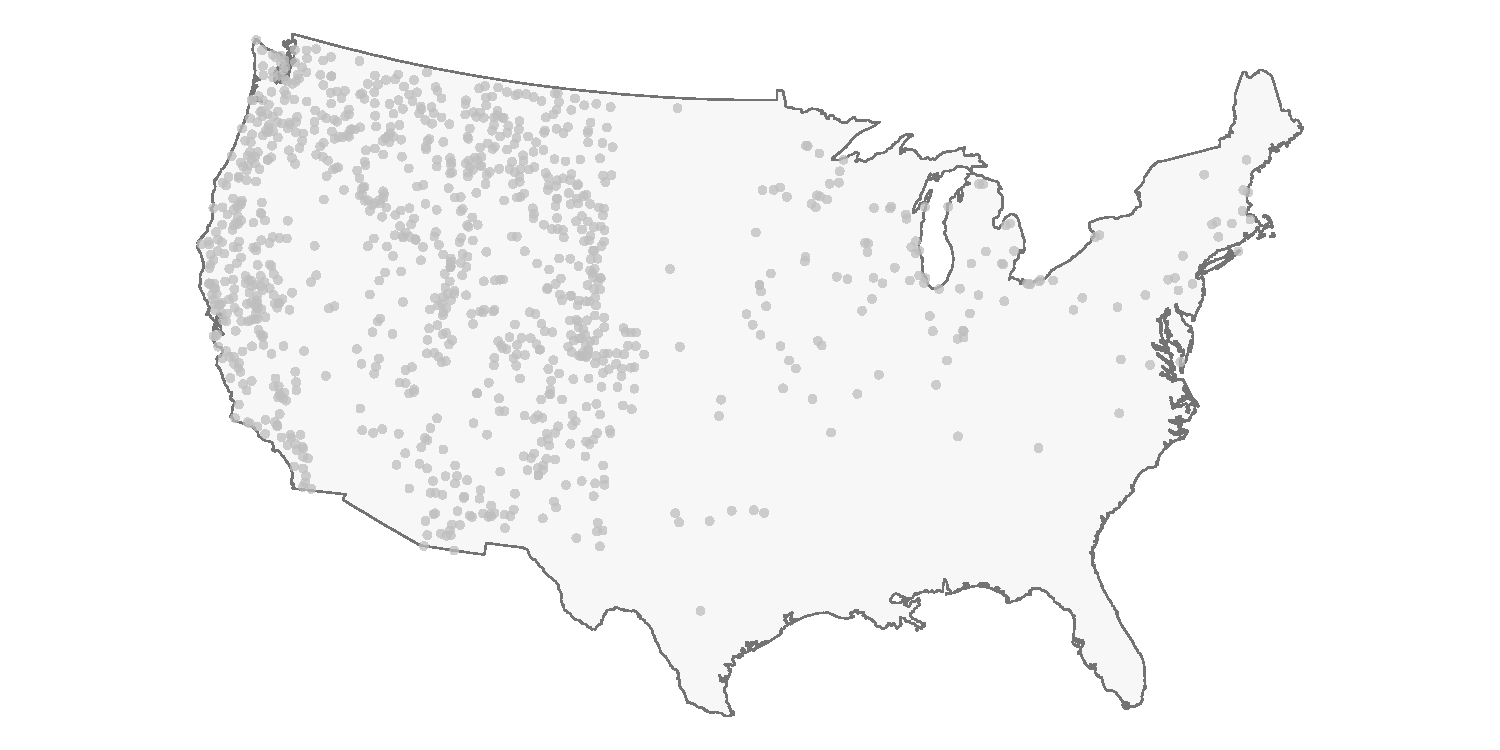
\includegraphics[width=0.9\textwidth]{../figure-latex/observation_locations.pdf}
\caption{Locations of sites in the historic lilac-honeysuckle dataset used to fit the model.}
\label{fig:observation_locations}
\end{figure*}


\begin{figure*}
\centering
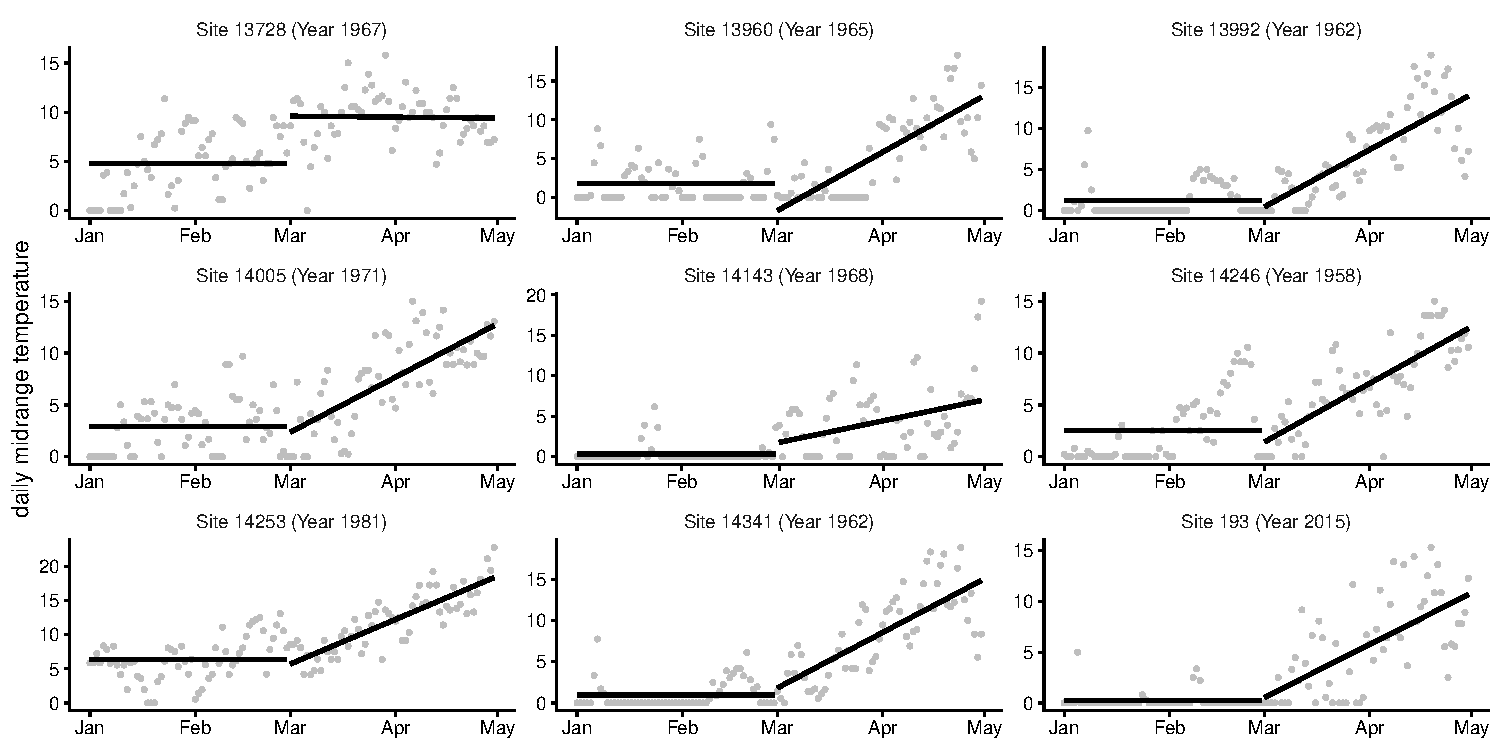
\includegraphics[width=0.9\textwidth]{../figure-latex/temp_plots-1.pdf}
\caption{Springtime daily midrange temperatures (points) with \(\alpha\)
(mean from Jan to Feb) and \(\beta\) (slope from Mar to Apr) for nine
randomly selected sites from lilac-honeysuckle dataset (Rosemartin et al. 2015) as measured by 
GHCND stations nearby. Temperatures below 0 are set to 0.}
\label{fig:temp_plot-1}
\end{figure*}

\begin{figure*}
\centering
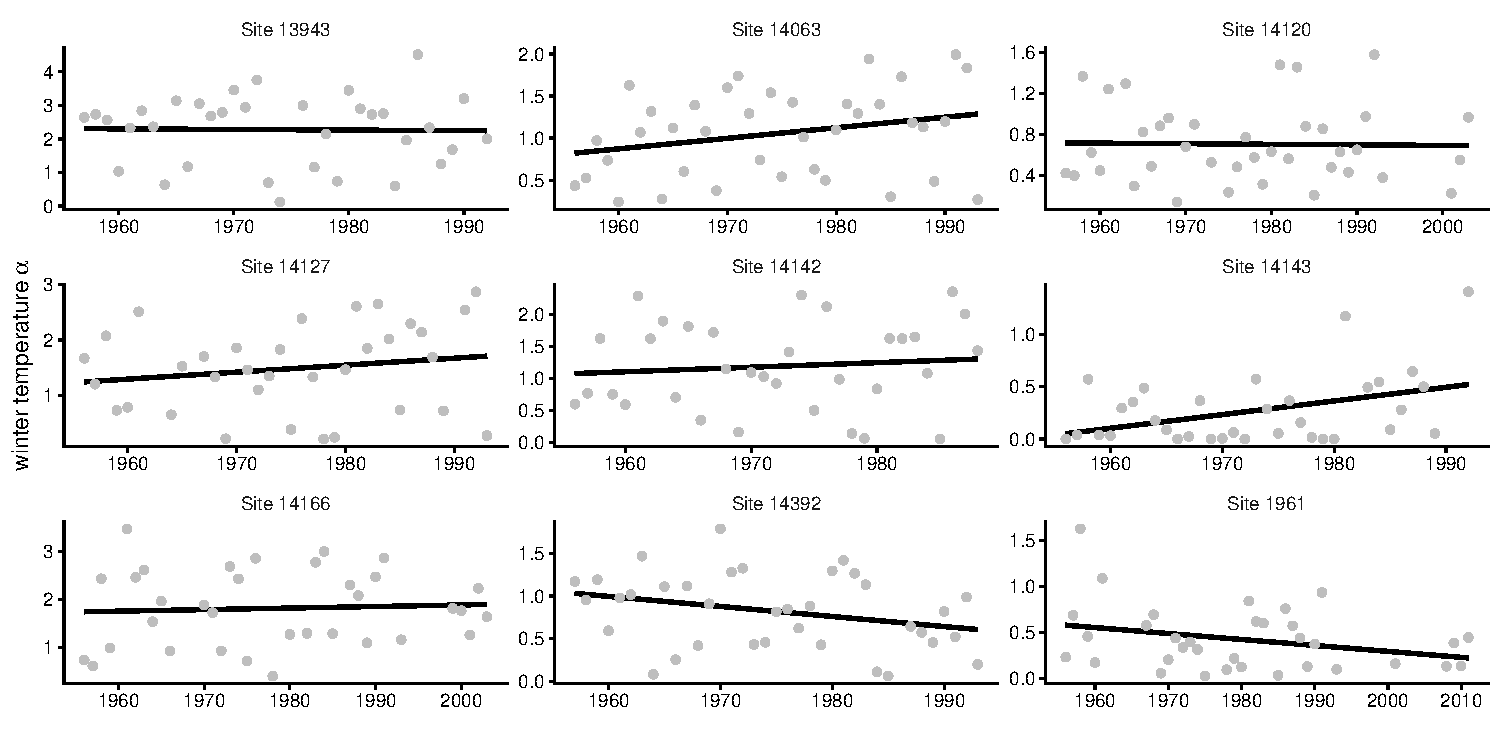
\includegraphics[width=0.9\textwidth]{../figure-latex/alpha_plots-1.pdf}
\caption{Changes in \(\alpha\) for the nine sites from lilac-honeysuckle data (Rosemartin et al. 2015) with 
longest running records as as measured by GHCND stations nearby. Trend line calculated using linear regression.}
\label{fig:temp_alpha}
\end{figure*}

\begin{figure*}
\centering
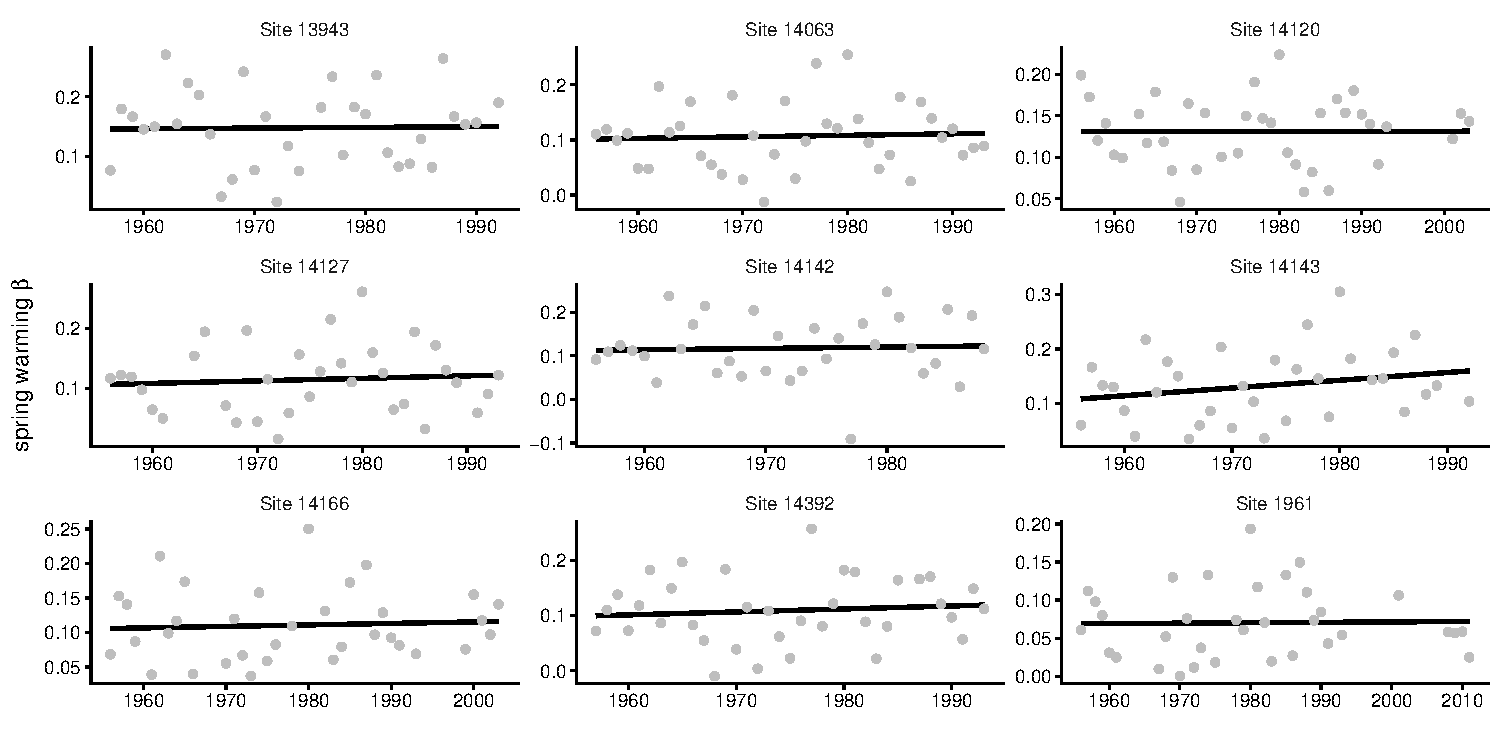
\includegraphics[width=0.9\textwidth]{../figure-latex/beta_plots-1.pdf}
\caption{Changes in \(\beta\) for the nine sites from lilac-honeysuckle data (Rosemartin et al. 2015) with 
longest running records as as measured by GHCND stations nearby.  Trend line calculated using linear regression.}
\label{fig:temp_beta}
\end{figure*}

\vfill

\begin{figure*}
\centering
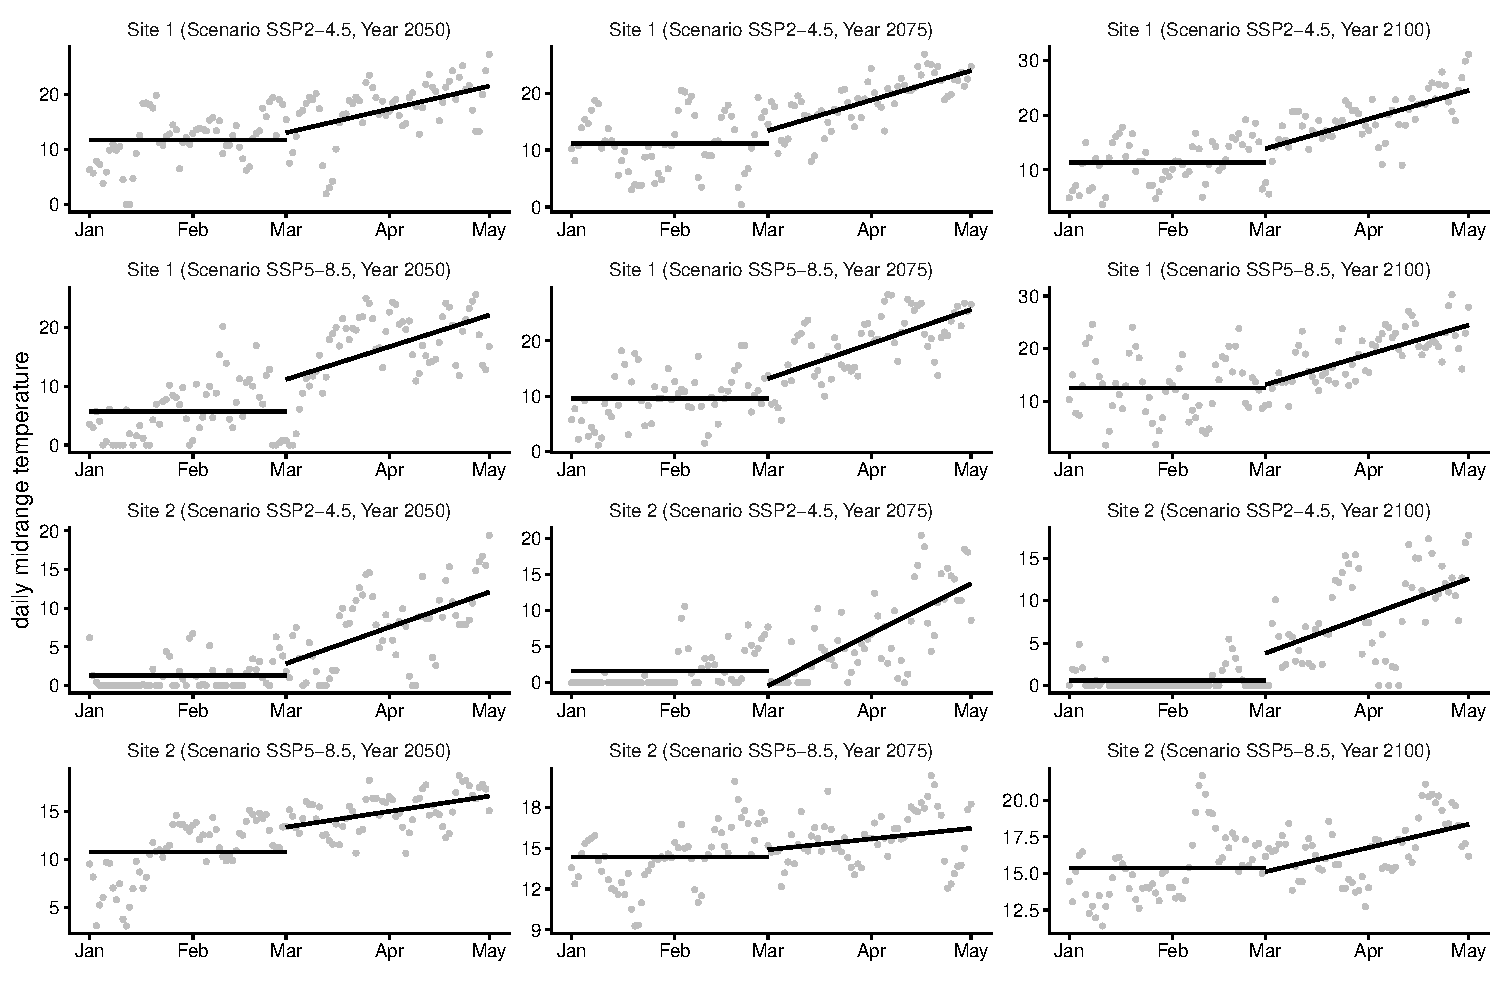
\includegraphics[width=0.9\textwidth]{../figure-latex/temp_plots-2.pdf}
\caption{Springtime daily midrange temperatures (points) with \(\alpha\)
(mean from Jan to Feb) and \(\beta\) (slope from Mar to Apr) for two randomly selected sites under two scenarios for the years 2050, 2075, and 20100 from the NEX-GDDP-CMIP6 dataset (Thrasher et al. 2022). Temperatures below 0 are set to 0.}
\label{fig:temp_plot-2}
\end{figure*}

\vfill

\begin{figure*}
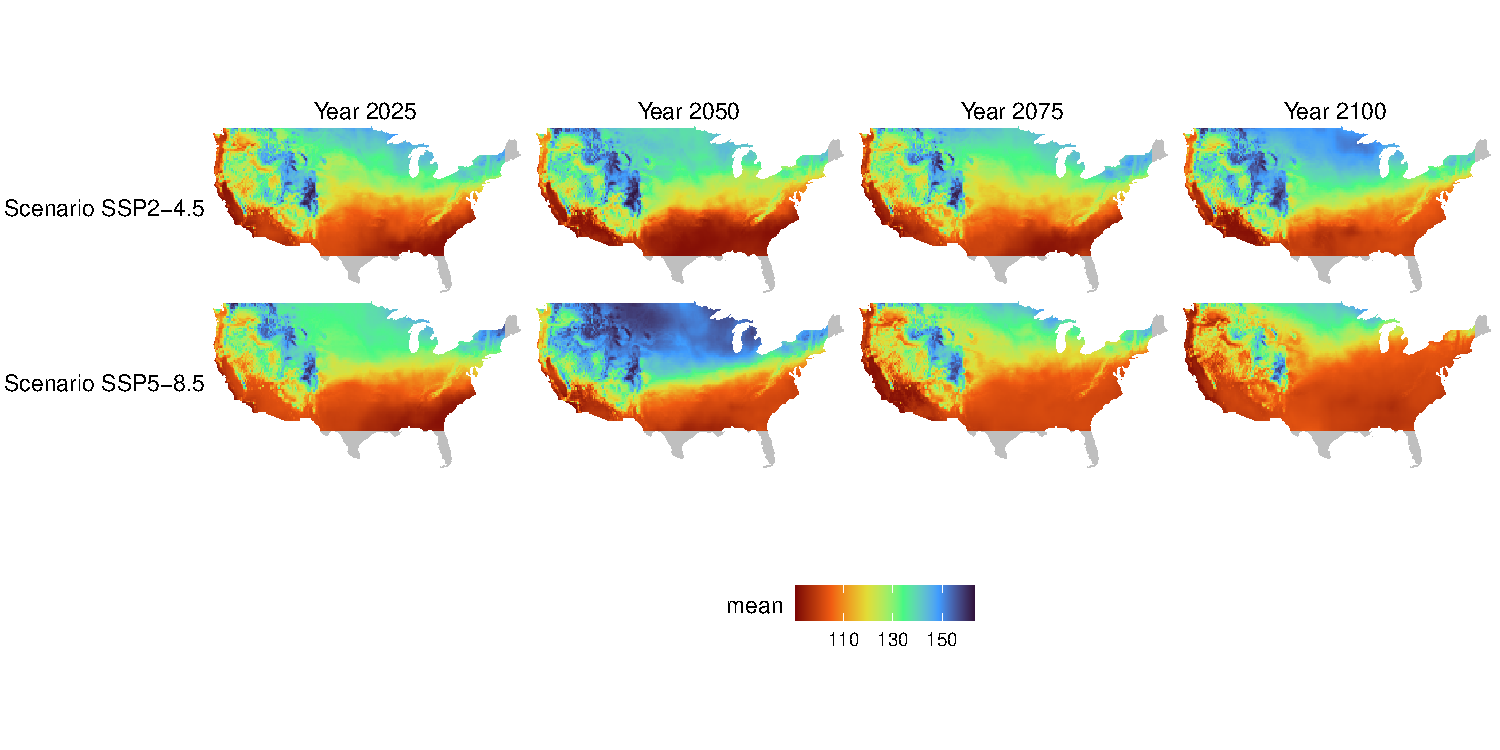
\includegraphics[width=1\linewidth]{../figure-latex/forecast_mean} \caption{Predicted mean of lilac bloom dates in years 2025, 2050, 2075, and 2100 (columns) across the continental United States under temperatures projected under two scenarios (rows) from NEX-GDDP-CMIP6 \citep{thrasher2022nasa} in which additional warming is moderate (top) or high (bottom). Lighter areas indicate earlier blooms due to higher temperatures. Under SSP2-4.5, the mean bloom date is largely constant between 2050 and 2100, while under SSP5-8.5, the mean bloom date advances moderately.}
\label{fig:forecast_mean}
\end{figure*}

\begin{figure*}
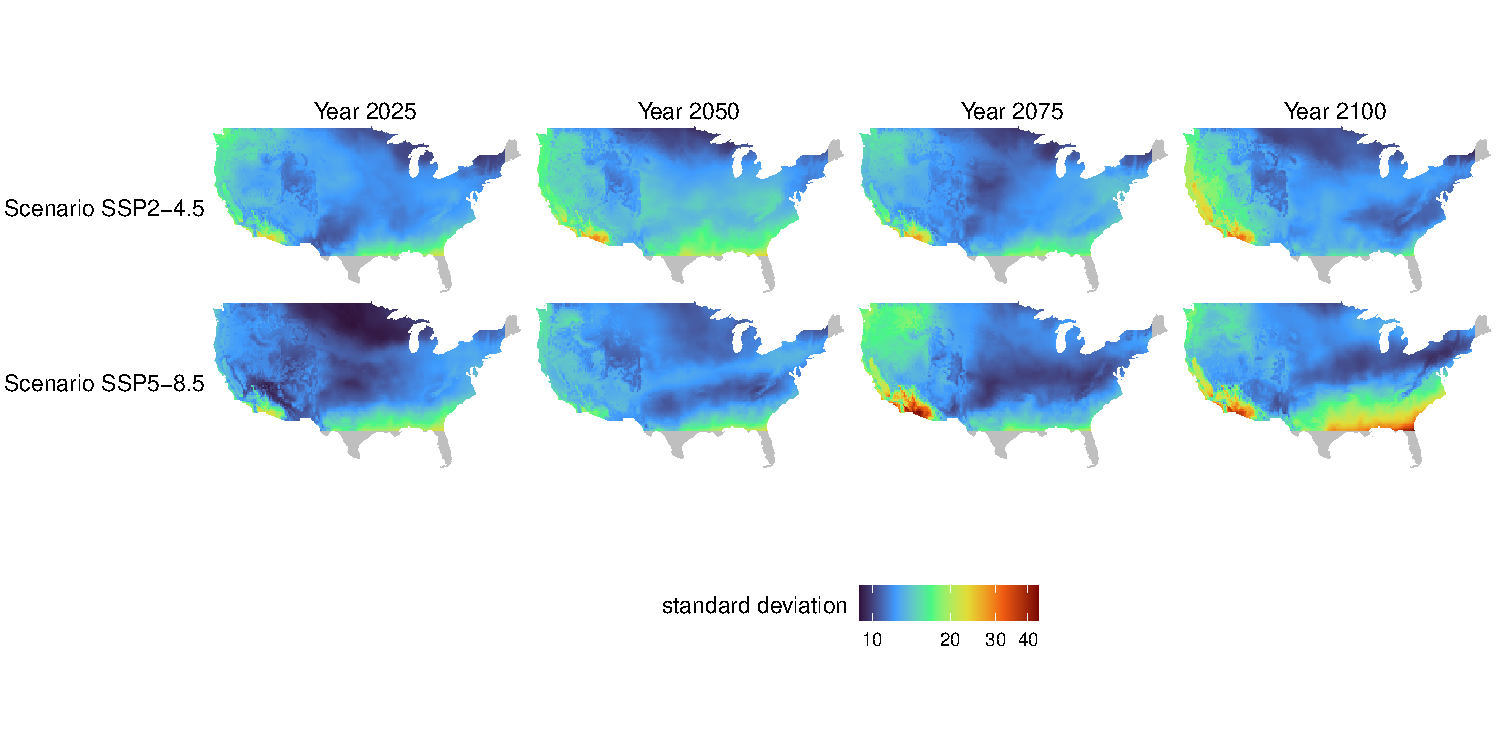
\includegraphics[width=1\linewidth]{../figure-latex/forecast_var} \caption{Predicted standard deviation of lilac bloom dates in years 2025, 2050, 2075, and 2100 (columns) across the continental United States under temperatures projected under two scenarios (rows) from NEX-GDDP-CMIP6 \citep{thrasher2022nasa} in which additional warming is moderate (top) or high (bottom). Light areas indicate more variation (less synchrony) due to higher temperatures. Under SSP2-4.5, the standard deviation is largely constant between 2050 and 2100, while under SSP5-8.5, the standard deviation increases dramatically, particularly in the Southeast and Southwest. These dramatic increase is due to a regime change, which we refer to as a `scattered spring.'}
\label{fig:forecast_var}
\end{figure*}

\newpage

\subsection*{SI.6 Simulations}\label{si-simulations}

We run two simulations to verify the interpretation of our findings. The
first verifies the asymptotic approximation of the thermal-sum model derived in Section A.1. 
The second verifies the interpretation of the data in Section A.2.

\subsubsection*{Simulation 1}\label{simulation-1}

We verify the accuracy of the two asymptotic normal
approximations for the hitting time \[
\nu(\tau)=\min\Big\{n\ge 1:\ \sum_{i=1}^n X_i>\tau\Big\}
\] under the model \[
X_i=\alpha+\beta i+\varepsilon_i,\qquad \varepsilon_i\sim \mathrm{Normal}(0,\sigma^2).
\]

We set \(\sigma=20\) and generate daily temperatures
until the threshold \(\tau\) is reached, recording the corresponding
hitting time \(\nu(\tau)\). We repeat this procedure \(R=10{,}000\) times
for thresholds \(\tau = \{1000,2000\}\), \(\alpha = \{2, 4\}\) and
\(\beta = \{0, 0.1 \}\). When \(\beta = 0\), the simulation matches the
winter regime, and when \(\beta = 0.1\), it matches the spring regime.

We then compare these simulations with the corresponding asymptotic distribution.
When \(\beta=0\), we use the distribution \[
\nu(\tau)\ \dot{\sim}\ \mathrm{Normal}\!\left(\frac{\tau}{\alpha},\ \frac{\sigma^2 \tau}{\alpha^3}\right).
\] When \(\beta>0\), we use the distribution \[
\nu(\tau)\ \dot{\sim}\ \mathrm{Normal}\!\left(\sqrt{\frac{2\tau}{\beta}}-\frac{\alpha}{\beta}+\frac12,\ 
\frac{\sigma^2}{\beta^{3/2}\sqrt{2\tau}}\right).
\]

The simulated distribution of \(\nu(\tau)\) is represented in Figure \ref{fig:simulations}
below by the histograms, where we have standardized by subtracting the mean and dividing by the standard deviation of the 
corresponding asymptotic distribution. Overlaid is the standard normal density. Across both regimes, the standardized 
histograms align closely with the \(\mathrm{Normal}(0,1)\) curve, and the agreement improves as \(\tau\)
increases, providing a visual confirmation of the derived asymptotic
distributions.

\begin{figure*}
\centering
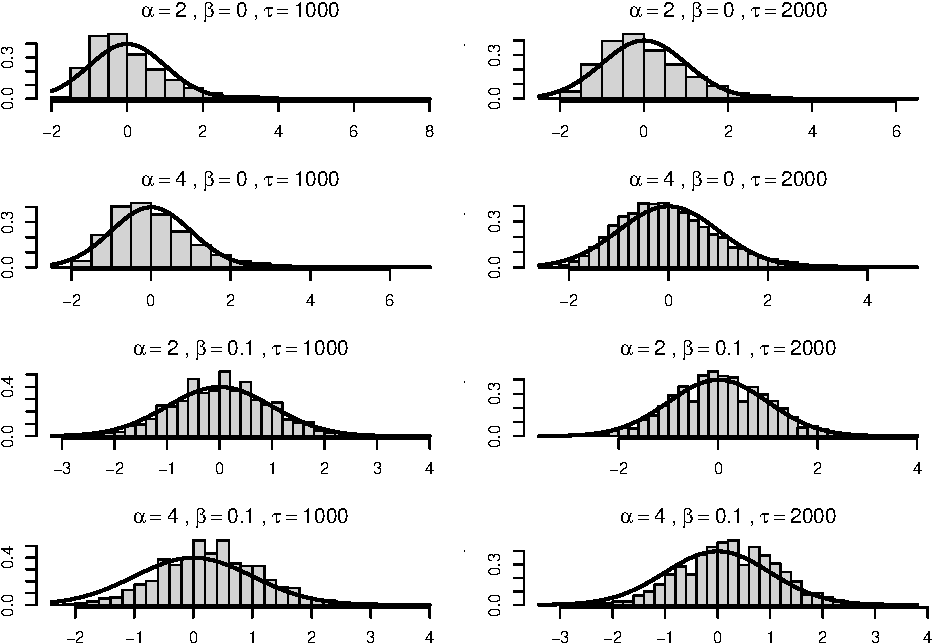
\includegraphics[width=0.9\textwidth]{../figure-latex/simulation1-1.pdf}
\caption{Simulations comparing the distribution of bloom dates (histogram) with an asymptotic approximation (solid line) under two regimes: winter (top two rows) and 
spring (bottom two rows).}
\label{fig:simulations}
\end{figure*}

\subsubsection*{Simulation 2}\label{simulation-2}

To verify our interpretation of the data, we simulate daily temperatures \[
X_i=\mu_i+\varepsilon_i,\qquad \varepsilon_i\sim \mathrm{Normal}(0,\sigma^2),
\] with \(\sigma=20\), where the deterministic component follows \[
\mu_i=
\begin{cases}
\alpha, & i=1,\dots,90 \quad \text{(January--February)},\\[2pt]
\alpha+\beta(i-90), & i=91,\dots,180 \quad \text{(March--April)}.
\end{cases}
\] Bloom occurs when cumulative temperature first exceeds a threshold
\(\tau\), i.e. \[
\nu(\tau)=\min\Big\{n\ge 1:\ \sum_{i=1}^n X_i>\tau\Big\}.
\] We simulated \(R=10{,}000\) independent realizations of \(\nu(\tau)\)
for each combination of \(\alpha\in\{4,8,10\}\),
\(\beta\in\{0.2,0.4,0.8\}\), and \(\tau\in\{1000,2000\}\).
We report the mean (left) and standard deviation (right) of \(\nu(\tau)\)
in Tables \ref{tab:sim_mean_1000}-\ref{tab:sim_sd_2000},
arranged with rows indexing \(\alpha\) and columns indexing \(\beta\).

The results reproduce the trends observed in the lilac
data. Mean bloom dates decrease as either
\(\alpha\) increases or \(\beta\) increases
(Tables \ref{tab:sim_mean_1000} and
\ref{tab:sim_mean_2000}). Within a fixed \(\alpha\) row, increasing
\(\beta\) reduces the standard deviation of bloom dates
(Tables \ref{tab:sim_sd_1000} and
\ref{tab:sim_sd_2000}), consistent with the prediction that
increasing average temperatures diminish the influence of noise on the
threshold-crossing time. Holding \(\beta\) fixed, the standard deviation is often
larger at higher \(\alpha\) (particularly for \(\beta\in\{0.4,0.8\}\)),
consistent with the prediction that earlier crossings
occur in a flatter portion of the seasonal cycle where microclimate
variability has greater influence.

\begin{table*}[t]
\centering
\caption{Simulated mean and standard deviation of the bloom date
$\nu(t)$ across $R=10{,}000$ replicates with thresholds $\tau\in\{1000,2000\}$. Rows denote the winter
temperature ($\alpha$), and columns denote spring warming ($\beta$).}
\label{tab:sim_piecewise_all}

\setlength{\tabcolsep}{6pt}
\renewcommand{\arraystretch}{1.15}

\begin{minipage}{0.49\linewidth}
\centering
\subcaption{mean, $\tau=1000$}
\label{tab:sim_mean_1000}
\begin{tabular}{lrrr}
\toprule
$\alpha$ $\backslash$ $\beta$ & 0.2 & 0.4 & 0.8 \\
\midrule
4  & 151.66 & 136.83 & 124.86 \\
8  & 114.87 & 111.27 & 106.85 \\
10 &  98.45 &  97.20 &  95.72 \\
\bottomrule
\end{tabular}

\vspace{1.0em}


\subcaption{mean, $\tau=2000$}
\label{tab:sim_mean_2000}
\begin{tabular}{lrrr}
\toprule
$\alpha$ $\backslash$ $\beta$ & 0.2 & 0.4 & 0.8 \\
\midrule
4  & 199.54 & 171.15 & 149.16 \\
8  & 169.81 & 152.43 & 137.37 \\
10 & 156.22 & 143.40 & 131.34 \\
\bottomrule
\end{tabular}

\end{minipage}
\hfill
\begin{minipage}{0.49\linewidth}
\centering
\subcaption{sd, $\tau=1000$}
\label{tab:sim_sd_1000}
\begin{tabular}{lrrr}
\toprule
$\alpha$ $\backslash$ $\beta$ & 0.2 & 0.4 & 0.8 \\
\midrule
4  & 15.48 & 10.42 &  7.21 \\
8  & 16.53 & 13.27 & 10.50 \\
10 & 15.94 & 14.45 & 12.71 \\
\bottomrule
\end{tabular}
\vspace{1.0em}

\subcaption{sd, $\tau=2000$}
\label{tab:sim_sd_2000}
\begin{tabular}{lrrr}
\toprule
$\alpha$ $\backslash$ $\beta$ & 0.2 & 0.4 & 0.8 \\
\midrule
4  & 10.96 & 7.22 & 4.84 \\
8  & 10.93 & 7.50 & 5.11 \\
10 & 10.69 & 7.66 & 5.36 \\
\bottomrule
\end{tabular}
\end{minipage}
\end{table*}


\newpage

%%%  REFERENCES: As of 2023, all Cell Press journals 
%%%  use Numbered (AMA) style. We recommend placing 
%%%  your references in the included "references.bib" 
%%%  file.


\bibliography{si_auerbach_gelman_wolkovich}

\end{document}
